\documentclass[12pt]{article}

\usepackage{fancyhdr}
\usepackage{hyperref}
\usepackage{xcolor}
\usepackage{pdfpages}
\hypersetup{
	colorlinks=true,
	linkcolor=blue
}

\setlength{\headheight}{14.49998pt}
\addtolength{\topmargin}{-2.49998pt}

\title{\bf{Software Engineering Project}}
\author{\bf{DispatchNet:} \\ Alessio Zanon \\ Leonardo Tonetta \\ Luca Fiorini}
\date{\it{Use Case Analysis}}

\pagestyle{fancy}
\fancyhead[l]{DispatchNet}
\fancyhead[c]{Project TRE}
\fancyhead[r]{v1.2}
\fancyfoot[c]{\thepage}

\makeatletter
\renewcommand*{\numberline}[1]{\hb@xt@5em{#1\hfil}} 
\makeatother

\makeatletter
\NewExpandableDocumentCommand{\mynumbering}{m}{%
  \ExpandArgs{c}\@mynumbering{c@#1}%
}
\ExplSyntaxOn
\NewExpandableDocumentCommand{\@mynumbering}{m}
 {
  \int_case:nn { #1 }
   {
    {0}{0}
    {1}{1}
    {2}{2}
    {3}{3}
    {4}{4}
    {5}{O }
    {6}{FR }
    {7}{NFR }
    %...
   }
 }
\ExplSyntaxOff

\renewcommand{\thesection}{\mynumbering{section}}


\renewcommand\bf[1]{\textbf{#1}}
\renewcommand\it[1]{\textit{#1}}
\newcommand\un[1]{\underline{#1}}
\newcommand\hyl[1]{\hyperref[#1]{#1}}
\newcommand\subs[2]{\subsection{#1}\label{#2}}
\newcommand\ssubs[2]{\subsubsection{#1}\label{#2}}
\newcommand\imgarg[2]{\begin{center}{\footnotesize\includegraphics[width=#2\textwidth]{#1}\newline Original image in our \href{https://github.com/DispatchNet/TRE/blob/uc/D2_DispatchNet/#1}{Github}}\end{center}} %Remember to switch away from "uc" to "main" when the merge happens
\newcommand\imgins[1]{\imgarg{#1}{0.65}}
\newcommand\uclnk[4]{
	%\newpage\subsubsection{#1} #4 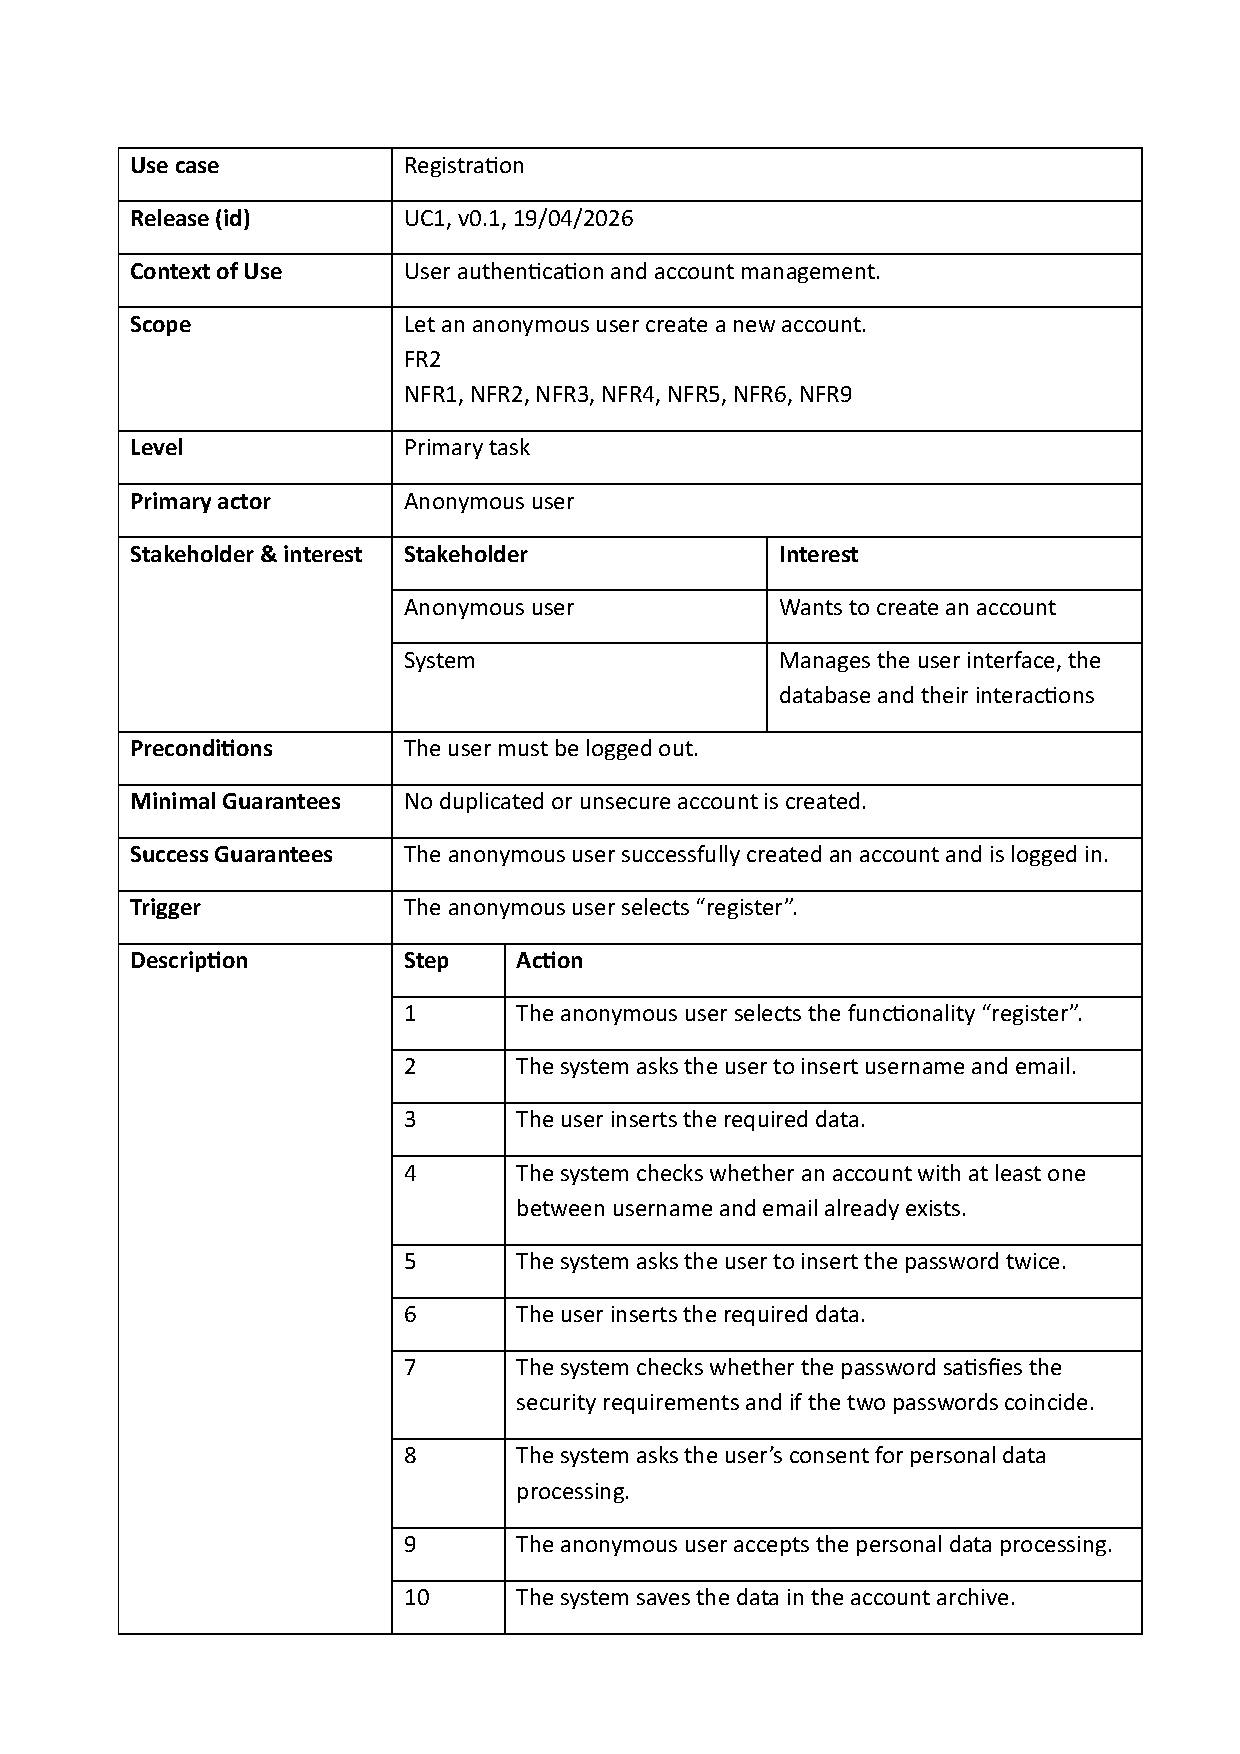
\includepdf[pages={#2}, linktodoc=true]{use_cases/use_cases_v0.5.pdf}\imgarg{activity_diagrams/UC#3_activity.pdf}{0.6} \imgarg{sequence_diagrams/UC#3_sequence.pdf}{1}
	}

\begin {document}
\maketitle

\newpage
\tableofcontents \label{Contents}

\section*{Readability notes}
\bf{Bold} words are system-important constructs. \newline
\un{Underlined} nouns are actors of the system. \newline
\it{Italic} words are special keywords to denote important limits of the project. \newline
\hyperref[Contents]{Hyperlinks} in reference to sections and subsections will be blue. \newline
\href{https:\\www.google.com}{Hyperlinks} to external web content will be in magenta. \newline
\textcolor{green}{Green text} is text in D1 added or modified for D2

\newpage

\addcontentsline{toc}{section}{Purpose}
\section*{Purpose}
This document describes the use cases, their relation, and the class-based diagram of Project "TRE", which implements a rail transport management system.

The purpose of this document is to: 
\begin{itemize}
	\item Represent all intended use cases
	\item Relate use cases with eachother and with stakeholders
	\item Itemize and relate the major data-components employed by the system
	\item Provide a top-level view of the system's operations
\end{itemize}

\newpage

\addcontentsline{toc}{section}{RE: Objectives}
\section*{RE: Objectives}

A major European rail infrastructure manager received an idea for a unified rail service scheduling and ticketing system, and has chosen us to prototype a trial run, over multiple regions in their network.\\

Thus, the project provides a platform that covers the needs of both \un{passengers} and \un{train companies}, as well as an underlying 
management system of any regional-sized rail network, which supports \un{network managers} in its administration. \\
It provides a set of functionalities which support the planning of train travel. The system lets \un{passengers} discover paths, view scheduling and manage tickets. On the other side, it lets \un{train companies} introduce train services and \un{network managers} administer the network.\\
The project coordinates the functionalities for each stakeholder into a solution that has been identified in an application accessible for the aforesaid users. \\

\noindent The main objectives of the project are:

\subsection*{Ticketing system}
\addcontentsline{toc}{subsection}{Ticketing system}
Subsystem which deals with tickets, from the search to the possible actions after the purchase. 
It includes basic operations that the \un{passenger} can perform, such as:
\begin{itemize}
	\item Viewing tickets details.
	\item Purchase.
	\item Accessing tickets history.
	\item Cancellation.
\end{itemize}

% \it{Boundary:} The project assumes the use of a third-party \un{payment gateway} system, implementing only a place-holder for a real 
% integration with it.

\subsection*{Route-finding}
\addcontentsline{toc}{subsection}{Route-finding}
The system shall let \un{passengers} select a starting station, a destination station, and either a departure time or arrival time.\\
It computes and ranks possible \bf{routes} that best fit the user's request and permissions
(for example, not permitting cargo trains to \un{passengers}).\\
The user must be able to compare the options based on:
\begin{itemize}
    \item Departure and arrival times.
    \item Number of transfers.
    \item Possible transfer locations.
\end{itemize}

\subsection*{Virtual board}
\addcontentsline{toc}{subsection}{Virtual board}
The system provides \un{passengers} access to departure and arrival boards for any station. It also shows intermediate stations and scheduled times for each 
individual train service.

\subsection*{Rail system modeling}
\addcontentsline{toc}{subsection}{Rail system modeling}
The system provides a data-driven approach to rail network modelling, supporting an efficient administration of the infrastructure.\\
It shall support:
\begin{itemize}
    \item Management of the network by the \un{network manager}.
    \item Management of rolling stock by the \un{network manager}.
    \item Submission of a new service request by \un{train companies}.
    \item Review of a service request by the \un{network manager}.
\end{itemize}

\newpage

\phantomsection
\addcontentsline{toc}{section}{RE: Stakeholders}
\section*{RE: Stakeholders}

\addcontentsline{toc}{subsection}{Internal}
\subsection*{Internal}

\addcontentsline{toc}{subsubsection}{Human}
\subsubsection*{Human}
\un{Network managers:}, the product owner. They manage the rail network combining the availability of \un{train companies} with \un{passengers'} needs.\\
They are the primary stakeholders for making functional decisions.

\addcontentsline{toc}{subsubsection}{Human}
\subsubsection*{Non-Human}
\un{Database}, where all the information used by the application are stored.

\addcontentsline{toc}{subsection}{External}
\subsection*{External}

\addcontentsline{toc}{subsubsection}{Human}
\subsubsection*{Human}
\un{Passengers}, the main end users. They want to streamline their interactions with the train transport system, including:
\begin{itemize}
	\item Searching for routes and schedules.
	\item Analyzing departure/arrival boards as well as train information.
	\item Purchasing tickets.
\end{itemize}

\noindent\un{Train companies}, who provide the rolling stock. They request the introduction of services. They are also expected to provide information of trains they ask to be managed.

\noindent\un{Anonymous users}, who have not yet authenticated. They are considered as passengers with restricted access to functionalities that require authentication.

\addcontentsline{toc}{subsubsection}{Non-human}
\subsubsection*{Non-human}
\un{Payment gateway}, which provides the underlying payment methods.\\

% \it{Boundary:} The project will not provide actual transactions nor integration with any payment application.

\newpage

\addcontentsline{toc}{section}{Component Diagram}
\section*{Component Diagram}
\begin{center}
	\footnotesize
	\imgarg{components/components_diagram.pdf}{1}
	Original image can be found on our \gitter{components/components_diagram.pdf}
\end{center}

\subsection*{User authentication}
\addcontentsline{toc}{subsection}{User authentication}
\imgins{components/user_authentication_component.pdf}
\uclnk{Registration}{1-3}{01}{}
\uclnk{Login}{14-15}{06}{}
\uclnk{Logout}{16}{07}{}

\subsection*{User management}
\addcontentsline{toc}{subsection}{User management}
\imgins{components/user_management_component.pdf}
\uclnk{Account deletion}{4}{02}{}
\uclnk{Account data view}{5}{03}{}
\uclnk{Account data change}{6-9}{04}{}
\uclnk{Reset password}{10-13}{05}{}

\subsection*{Ticketing management}
\addcontentsline{toc}{subsection}{Ticketing management}
\imgins{components/ticketing_management_component.pdf}
\uclnk{View Ticket Details}{17}{08}{}
\uclnk{Ticket purchase}{18-19}{09}{}
\uclnk{Ticket cancellation}{20-21}{10}{}
\uclnk{Ticket history}{22}{11}{}

\subsection*{Path finding}
\addcontentsline{toc}{subsection}{Path finding}
\imgins{components/ticketing_management_component.pdf}
\uclnk{Find Path}{23-24}{12}{}
\uclnk{Purchase Tickets in path}{25-26}{12.1}{}
\uclnk{View Stations in path}{27}{12.2}{}

\subsection*{Info view}
\addcontentsline{toc}{subsection}{Info view}
\imgins{components/ticketing_management_component.pdf}
\uclnk{View Train and Station Details}{28-29}{13}{}
\uclnk{Search Info}{30-31}{14}{}
\uclnk{View Map}{32}{15}{}

\subsection*{Network management}
\addcontentsline{toc}{subsection}{Network management}
\imgins{components/network_management_component.pdf}
\uclnk{View Network Elements}{33}{16}{}
\uclnk{Insert Station Data}{34}{17}{}
\uclnk{Insert Junction Data}{35}{18}{}
\uclnk{Insert Line Data}{36}{19}{}
\uclnk{Create Station}{37}{20}{}
\uclnk{Create Junction}{38}{21}{}
\uclnk{Create Line}{39}{22}{}
\uclnk{Edit Station}{40}{23}{}
\uclnk{Edit Junction}{41}{24}{}
\uclnk{Edit Line}{42}{25}{}
\uclnk{Delete Station}{43}{26}{}
\uclnk{Delete Junction}{44}{27}{}
\uclnk{Delete Line}{45}{28}{}

\subsection*{Service management}
\addcontentsline{toc}{subsection}{Service management}
\imgins{components/service_management_component.pdf}
\uclnk{Defining a Train Type}{46}{29}{}
\uclnk{Registering a Service Type}{47}{30}{}
\uclnk{Create Service Request}{48-49}{31}{}
\uclnk{Service Request Review}{50}{32}{}

\newpage

\phantomsection
\section*{Class Diagram}
\addcontentsline{toc}{section}{Class Diagram}
\begin{center}
	\footnotesize
	\imgarg{class_diagram/class_diagram.pdf}{1}
	Original image avaiable at our \gitter{D2_DispatchNet/class_diagram/class_diagram.pdf}
\end{center}
\subsection*{Description}

\bf{Main}: main class where all the management classes are instantiated

\bf{UserManagement}: used to manage the user module

addAnon: Create an anonymous user with unique ID and add it to the list. Necessary for UC2, 7
addAuth: Upgrade an anonymous user into an authenticated one, removing the former and adding the latter to respective lists. Necessary for UC1, 6
removeAnon: Delete an anonymous user from list
removeAutho: Remove an authenticated user from list. Necessary for UC2, 7

\bf{AnonymousUser}: unregistered user who can access the system without authentication 

register(): create a new account for UC1
resetPassword(): initiate the password reset process UC5
login(): become an authenticated user for UC6

\bf{AuthenticatedUser}: authenticated user who uses the system 

logout(): become an anonymous user for UC7

\bf{UserType}: classification of the user, implements FR1

\bf{NetworkManager}: authenticated user who manages the railway network, not an end user
(in the following <Template> is a shortcut for Station, Junction or Line, used just for a short description)
 
viewNetwork(): view the network graph UC16
create<Template>(): create a new <Template> UC20, 21, 22
edit<Template>(<Template>): modify <Template> data UC23, 24, 25
delete<Template>(<Template>): remove a <Template> from the network UC26, 27 28
reviewServiceRequest(ServiceRequest): review a service request submitted by a train company UC32

\bf{EndUser}: authenticated user 
who uses the end functionalities of the application
 
deleteAccount(): for UC2
viewData(): view personal account data UC3
changeData(): modify account data for UC4

\bf{Passenger}: authenticated user 
who directly uses the train
services
 
tickets: list of tickets owned by the passenger
findPath(): initiate a path search between stations for UC12
searchStationTrain(): search for a train or station by name for UC14
viewMap(): view the network map for UC15
purchaseTicket(Ticket): buy an individual ticket for UC9, UC12.1
purchaseTicket(GroupPass): buy a group pass for UC9
cancelTicket(Ticket): cancel an individual ticket for UC10
cancelTicket(GroupPass): cancel a group pass for UC10
getTicketsHistory(): view purchased and cancelled tickets for UC11

\bf{TrainCompany}: authenticated user who represents a train company 
createServiceRequest(): submit a new request for a service 
For UC31
createServiceType(): create a Service type
For UC30
createTrainType(): create a Train type
For UC29

\bf{Ticket}: A representation of a passenger trip between two stations, it is used to represent possible trips as well as representing a booking.

owner: passenger who owns the ticket
departure: The Departure this ticket starts from
lastStep: the ServiceStep this ticket's validity ends
getCost(): Compute the cost associated with this ticket (in cents)
For UC8,UC9,UC10,UC12
getEnd(): Get the end junction for this ticket
For UC8

\bf{GroupPass}: group ticket

owner: passenger who bought the pass
subTickets: list of tickets included in the pass

\bf{Pathfinding}: 
A class of objects representing an in-use pathfinding search. The results of the search are stored each as a list of stations and the tickets that would connect them

results: Storage of all results computed at construction, only accessed by srtPth()
constructor(): Explicitly mentioned since it populates the internal fields and computes the possible paths, while other methods modify the results field as requested by the User. Sets the factory-default in chosenSrt. For UC12
srtPth(): Takes the paths and ranks them based on the enum parameter, filtering the top results nondestructively. Uses the srtAlg enum to change behaviour based on a pre-set list of supported sorting decisions. For UC12
getResults(): Unlike other getters, calls srtPth to only provide the processed results, without permanently altering the variable (so that the sorting can be repeated without loss of data). For UC12 and UC12.2
prchTcks(): Uses getTcks on the same selected path (by index int) to perform UC 12.1

\bf{srtAlg}: The sorting algorithm to use

Length: Specified in FR14.1
Departure: Specified in FR14.2
Arrival: Specified in FR14.3
Cost: Specified in FR14.4

\bf{Network}: 
used to represent the network module; graph representation of the railway infrastructure infrastructure 

getJunctions(): get all junctions
For UC13 ,UC15
getLines(): get all lines
For UC13 ,UC15
addJunction(Junction):
For UC21,UC22
addLine(Line):
For UC22
removeJunction(Junction*):
For UC26,27 
removeLine(Line*):
For UC 28
existsWalk: verify whether a path exists between two Junctions used in UC12

\bf{Line}: undirected edge between two Junctions of the network, it's constructor implements UC19, 22

nTracks: number of tracks on the line
maxSpeed: maximum speed trains can achieve
getDetails(): provide a textual description of the object UC16

\bf{Junction}: Junction of the railway network. If station data exists it is not just a simple junction but additionally a station. It's constructor implements UC18, 21
 
lines: The lines connected to this junction
station: The optional station data associated to this junction
serviceSets: A set of unique services that pass through or stop at this junction. This is used to compute departures.
isStation(): True if this Junction is a station (I.E. It has station information)
getStation(): Get the station data
getDepartures(Time,Time): Compute and return a list of departures between given time criterion
For UC13,UC12
getLines(): return a list of pointers to the connected lines
getNeighbors(): return the neighboring Junctions via the connected lines
getDetails(): provide a textual description of the object
For UC16
addService(): Add a service that is known to stop at this junction.
For UC32

\b{fStationData}: Used to represent a station's data that may exist at a Junction (a Station is a Junction), It's constructor implements UC17, 20

platforms: A list of platforms
addPlatform(String):  Add a platform to the station if it doesn't already exist
For UC24
removePlatform(String): Remove an existing platform
For UC24
getDetails(): Provide a textual description for this element.
For UC13,UC16

\bf{ServiceStep}: one step of a service route. If stopData exists the service stops at this step

Junction: The Junction this step refers to
stopData: The stopping information if this service does stop at this step
travelMinutes: The time travelled
isStopping(): If the service is stopping, true, otherwise false

\bf{Departure}: A structure that holds a single departure's information
 
serviceSet: The ServiceSet that this departure references
serviceStep: The step of the ServiceSet this departure refers to
time: The time of the departure
getDetails(): Provide a textual description for this element
For UC13

\bf{StopData}: stopping details for a service step 

waitMinutes: minutes the service waits
platform: from which platform the passengers access the train

\bf{ServiceManagement}: used to manage the service module

\bf{ServiceRequest}: request to introduce a service, its constructor implements UC31 

serviceSet: serviceSet to be requested
approve(): approve the requested service
For UC32
reject(): reject the requested service
For UC32

\bf{ServiceSet}: a set of train services introduced by a train company
along a common route

operator: train company who introduced the service
steps: list of Junctions the service passes through
serviceType: ServiceType used by the ServiceSet
dispatches: A list of dispatches
that define when services originate from the first serviceStep.

\bf{ServiceStatus}: the status of a service

Effective: The service is operating
PendingApproval: The service is awaiting approval

\bf{Dispatch}: The dispatch information for an individual service

time: the time of departure from the first station in the ServiceSet
days: The days of the week this service operates 
trainNumber: This service's globally unique identifier
operatesOn(Weekday): Returns true if the service is operating on the given day of the week, otherwise false

\bf{ServiceType}: valid type of train service, its constructor implements UC30

pricePerKm: price per km (in cents)
getDetails(): returns a textual description of the object

\bf{TrainType}: specification of a train model, its constructor implements UC29

maxSpeed: maximum speed the train can achieve
isPassenger: true=passenger, false=cargo
seatedCapacity: number of seats
standingCapacity: number standing spots
getDetails(): provide a textual description of the object


\newpage


\addcontentsline{toc}{section}{Context Description (D1)}
\section*{Context Description (D1)}
Original, up-to-date file available on our \href{https://github.com/DispatchNet/TRE/blob/uc/D1_DispatchnNet/D1_DispatchNet.pdf}{Github}

\input{../D1_DispatchNet/D1_BodyText.tex}

\end {document}
